\PassOptionsToPackage{unicode}{hyperref}
\PassOptionsToPackage{hyphens}{url}
%
\documentclass[superscriptaddress, 12pt]{revtex4-2}%twocolumn
\usepackage{amsmath,amssymb}
\usepackage{iftex}
% Use upquote if available, for straight quotes in verbatim environments
\usepackage{xcolor}
\usepackage{subcaption}
%\usepackage{longtable}
\usepackage{booktabs,array}
\usepackage{multirow}
\usepackage{calc} % for calculating minipage widths
% Correct order of tables after \paragraph or \subparagraph
\usepackage{etoolbox}
\usepackage{footnote}
\usepackage{graphicx}
\usepackage{bookmark}
%\usepackage{babel}
\IfFileExists{xurl.sty}{\usepackage{xurl}}{} % add URL line breaks if available
\urlstyle{same}
\hypersetup{
  hidelinks,
  pdfcreator={LaTeX via pandoc}}
\usepackage{textgreek}
\usepackage{makecell}
\usepackage{multirow}
\usepackage{booktabs}
\usepackage[LGR,T1]{fontenc}
\usepackage[utf8x]{inputenc}
\usepackage{textalpha}
\usepackage{ulem}
\usepackage{textcomp}
\date{}


\begin{document}

\title{Influence of partial occupancy on the elastic tensor for FeCr \textsigma - phase.}

\author{Mariano Forti} \email{mariano.forti@icams.rub.de}
\affiliation{Interdisciplinary cetre for advanced materials simulations (ICAMS), Ruhr Universität Bochum, Germany}

\author{Thomas Hammerschmidt} \email{}
\affiliation{Interdisciplinary cetre for advanced materials simulations (ICAMS), Ruhr Universität Bochum, Germany}

\author{Guillaume Laplanche} \email{}
\affiliation{Ruhr Universität Bochum}


\maketitle

\section{Introduction}

The Fe-Cr system is an important alloy system with applications in structural and high-temperature environments. 
The \textsigma-phase can form at Cr concentrations between 45 and 50\%at and temperatures ranging from 550 to 800\textdegree ~\cite{laplanche_phase_2018} significantly influencing the mechanical properties of Fe-Cr alloys. 
Specifically, \textsigma-phase precipitation contributes to embrittlement and reduces corrosion resistance {\color{red}  [ref 2 detrimental sigma] }.
The \textsigma-phase unit cell is shown in \autoref{fig:sigmaUnitCell}. 
This is an intermetallic compound with a tetragonal structure (space group P4\textsubscript{2}/mnm) and exhibits complex atomic arrangements due to site-specific partial occupancies.  
Understanding its properties is essential for predicting its mechanical behavior and phase stability.  
There are different approaches to similar problems in atomistic simulations, based for instance on Density Functional Theory (DFT). 
Vesti et. al. ~\cite{vesti_ab-initio_2023} utilize a full sublattice model later averaged under an ideal mixing approximation to interpolate the properties of a W-Re \textsigma phase. 
Kabliman et. al. ~\cite{kabliman_ab_2012} use a mean field approximation to study several properties of the \textsigma phase in other binary systems, also based on full occupancy of the sublattices. 
This assumption may overlook local atomic configuration effects.  
In this work, we investigate how explicit consideration of partial occupancy influences the elastic properties of the \textsigma-phase through first-principles calculations. 
We focus on a Fe16Cr14 unit cell which can be modelled with nominal and on-site compositions in agreement with experimental observations.

\begin{figure}
  \subcaptionbox{\protect\label{fig:sigmaUnitCell}}{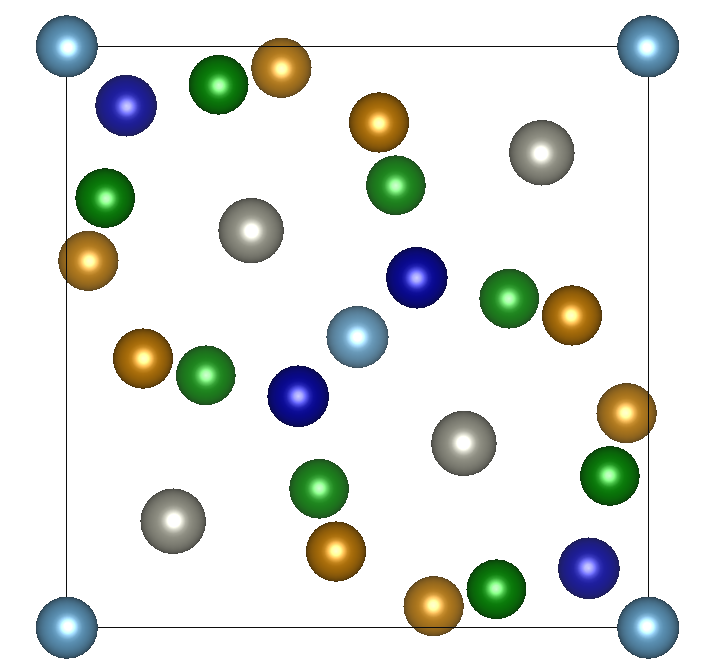
\includegraphics[height=4cm]{Figure_SigmaPhase001.png}}
  \caption{\protect\label{fig:introduction}
    (\subref{fig:sigmaUnitCell}) (001) view of the σ phase unit cell. Wyckoff sites are encoded in colors: 2a is light blue,
    4f in grey, 8i in green, 8i' in gold, 8j in blue. 
  }
\end{figure}

\section{Methodology}

We employ first-principles DFT calculations to determine the elastic constants of the Fe-Cr \textsigma-phase at a
nominal composition of Fe\textsubscript{16}Cr\textsubscript{14} (48\%at. Cr).  These calculations are conducted using
the Vienna Ab initio Simulation Package (VASP) ~\cite{Hafner_vasp}, utilizing the Perdew-Burke-Ernzerhof (PBE)
~\cite{Perdew1996} exchange-correlation functional and the Projector Augmented Wave (PAW) method ~\cite{Bloch1994,
kresse_ultrasoft_1999}.  The elastic tensor is derived from stress-strain relationships obtained via energy-strain
calculations


\paragraph{Full occupancy}

First, we calculate the properties of the \textsigma-phase using a full sublattice model. This means, that the lattice
positions of a WS are occupied either bu Cr or Fe. We calculate formation enthalpies and elastic constants for all the
possible configurations spanning the full composition range. 

\paragraph{Partial occupancy} To capture the impact of atomic disorder, we explicitly explore all possible atomic
arrangements within the \textsigma-phase unit cell, incorporating experimentally reported partial occupancies of Wyckoff
sites by Yakel~\cite{yakel_atom_1983} as reproduced in \autoref{fig:ExptPartialOccupancies}. However, the composition of
the 2a site would require a bigger unit cell to model accurately.  In order to keep the size of the simulation cell to
one unit cell, we consider two approximations to the partial occupancies, in both cases disregarding Cr occupation in
site 2a and rounding occupancies to integer numbers.  A first model, \autoref{fig:PartialOccupanciesA}, keeps one Fe
atom in the site 4f and 1 Cr atom in site 8i'.  In this conditions, the total number of possible configurations is $ 1
\times 4 \times \binom{8}{3}\times \binom{8}{1} \times \binom {8}{3} \approx 100k $, which are too many to consider dft
calculations of a significative sample. Then, we also consider a second model, \autoref{fig:PartialOccupanciesb}, which
keeps the same number of atoms in the 8i and 8j sites, while transferring the Cr atom from 8i' to 4f. This reduces the
number of possible configurations to $ 1 \times 1 \times \binom{8}{3}\times 1 \times \binom {8}{3} = 3136 $, which is a
more manageable number of configurations.

A subset of representative configurations is selected for detailed elastic constant
calculations. ~\cite{golesorkhtabar_elastic_2013}.

\begin{figure}
  \subcaptionbox{\protect\label{fig:ExptPartialOccupancies}}{\includegraphics[height=4cm]{example-image-a}}
  \subcaptionbox{\protect\label{fig:PartialOccupanciesA}}{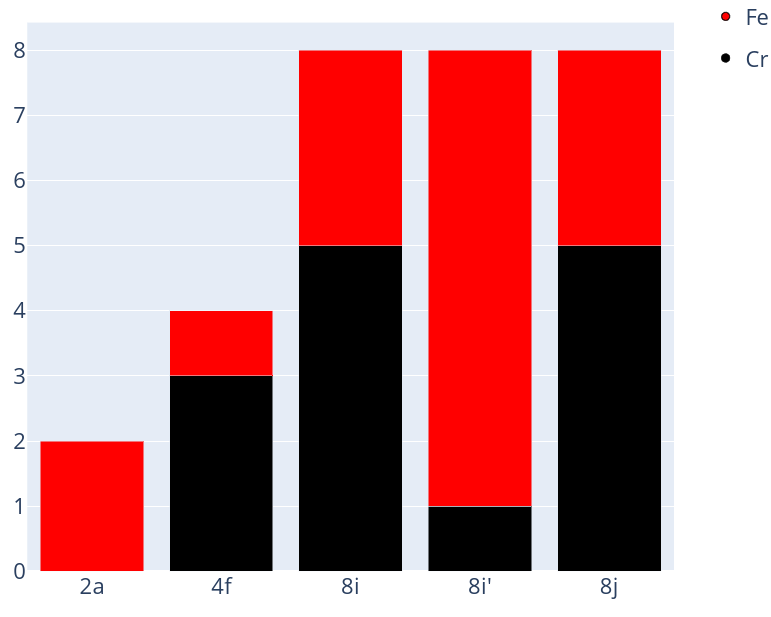
\includegraphics[height=4cm]{Figure_SigmaPhaseModelledPartialOccupancies_II.png}}
  \subcaptionbox{\protect\label{fig:PartialOccupanciesb}}{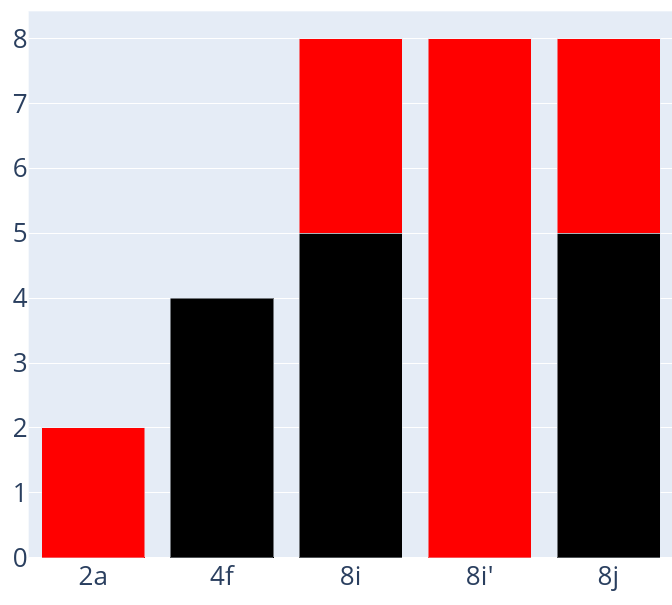
\includegraphics[height=4cm]{Figure_SigmaPhaseModelledPartialOccupancies.png}}

  \caption{\protect\label{fig:PartialOccupancies}
    (\subref{fig:ExptPartialOccupancies}) (001) view of the σ phase unit cell. Wyckoff sites are encoded in colors: 2a is light blue,
    4f in grey, 8i in green, 8i' in gold, 8j in blue. 
    (\subref{fig:PartialOccupanciesA}) First model of unit cell with partial occupancy, model B2\_A3B\_A5B3\_AB7\_A5B3.
    (\subref{fig:PartialOccupanciesB}) Further simplified model B2\_A3B2\_A5B3\_8B\_A5B3.
  }

\end{figure}

\section{Results}

Our results show that partial occupancy disrupts unit cell symmetry, significantly affecting the mechanical response of the \textsigma-phase. Unlike the widely used full sublattice model, which assumes high symmetry, explicit treatment of atomic disorder reveals some deviations in elastic constants. 
In a full sublattice model, the Fe-Cr \textsigma phase has a tetragonal unit cell in the space group P4\textsubscript{2}/mnm in the entire composition range. Fig. 1c) shows the calculated convex hull of formation enthalpies at 0K as a function of the Fe content. The positive enthalpies and the minima at around 40\%at Fe imply that the \textsigma phase might be stabilized by entropy or vibrational contributions, which are not considered here. In the other hand, introducing partial occupancies in Fe16Cr14 stabilizes the compound. However, the symmetry is broken, and the unit cell acquires a space group P.
Due to the low symmetry, the elastic tensor of the triclinic unit cell has 22 independent components, and their determination is computationally much more demanding than the full occupancy cases, requiring at least a hundred single point calculations for each sampled configuration. Fig 1d) shows a comparison of the calculated elastic tensor components to the expected values if the cell kept the symmetry. We see an overall deviation of around 10\%. 
Finally,  In Fig 1e) we report the changes in the VRH averaged elastic modulae with nominal composition and fractional occupation of the sublattices. We observe a slight stiffening of the compound for lower formation energies. 

\section{Conclusion}
In this work we are presenting a methodical study of the effects of partial occupancy in the properties of the \textsigma phase of the FeCr system. For the first time, the properties of this phase are explicitly calculated outside a full sublattice model. We observed a breakage of symmetry from a tetragonal to a triclinic unit cell, although the overall effect seems to be mild with deviations from expected values of around 10\%. By incorporating realistic atomic configurations based on partial occupancies, we provide a more precise description of the mechanical behavior of the Fe-Cr \textsigma-phase. These insights are essential for refining theoretical models and guiding experimental studies of intermetallic alloys.


\section{full occupancies}

\section{selection of working alloy}
final long term goal is CrMnFeCoNi (order by atomic number). We select the easiest binary with $\sigma$ phase. 
We select 16Fe14Fe because it was close to the experimental 50\%Fe and it is 
easy to distribute between the sublattices. 

show experimental partial occupancies, and the modelled distribnutions.
(there are slides)

explaining breaking of symmetry by partial occupancies with figures.


\bibliographystyle{naturemag} \bibliography{main.bib}

\end{document}
